
\subsection{Probability distributions, Markov kernels and string diagrams}

We make use of a string diagram notation for probabilistic reasoning. Graphical models are often employed in causal reasoning, and string diagrams are a particuarly rigorous graphical notation for probabilistic models. It comes from the study of Markov categories. Markov categories are abstract categories that represent models of the flow of information. We can form Markov categories from collections of sets -- for example, discrete sets or standard measurable sets -- along with the Markov kernel product as the composition operation. Markov categories come equipped with a graphical language of \emph{string diagrams}, and a coherence theorem which states that calid proofs using string diagrams correspond to valid theorems in \emph{any} Markov category \citep{selinger_survey_2010}. More comprehensive introductions to Markov categories can be found in \citet{fritz_synthetic_2020,cho_disintegration_2019}. Thus, while we limit ourselves to discrete sets in this paper, any derivation that uses only string diagrams is more broadly appliccable.

We say, given a variable $\RV{X}:\Omega\to X$, a probability distribution $\prob{P}^{\RV{X}}$ is a probability measure on $(X,\sigalg{X})$. Recall that a probability measure is a $\sigma$-additive function $\prob{P}^{\RV{X}}:\sigalg{X}\to [0,1]$ such that $\prob{P}^{\RV{X}}(\emptyset)=0$ and $\prob{P}^{\RV{X}}(X)=1$. Given a second variable $\RV{Y}:\Omega\to Y$, a conditional probability $\prob{Q}^{\RV{X}|\RV{Y}}$ is a Markov kernel $\prob{Q}^{\RV{X}|\RV{Y}}:X\kto Y$which is a map $Y\times \sigalg{X}\to [0,1]$ such that

\begin{enumerate}
    \item $y\mapsto \prob{Q}^{\RV{X}|\RV{Y}}(A|y)$ is $\sigalg{B}$-measurable for all $A\in \sigalg{X}$
    \item $A\mapsto \prob{Q}^{\RV{X}|\RV{Y}}{K}(A|y)$ is a probability measure on $(X,\sigalg{X})$ for all $y\in Y$
\end{enumerate}

In the context of discrete sets, a probability distribution can be defined as a vector, and a Markov kernel a matrix.

\begin{definition}[Probability distribution (discrete sets)]
A probability distribution $\prob{P}$ on a discrete set $X$ is a vector $(\prob{P}(x))_{x\in X}\in [0,1]^{|X|}$ such that $\sum_{x\in X} \prob{P}(x) = 1$. For $A\subset X$, define $\prob{P}(A)=\sum_{x\in A} P(x)$.
\end{definition}

\begin{definition}[Markov kernel (discrete sets)]
A Markov kernel $\prob{K}:X\kto Y$ is a matrix $(\prob{K}(y|x))_{x\in X,y\in Y}\in [0,1]^{|X||Y|}$ such that $\sum_{y\in Y} \prob{K}(y|x)=1$ for all $x\in X$. For $B\subset Y$ define $\prob{K}(B|x)=\sum_{y\in B}\prob{K}(y|x)$.
\end{definition}

In the graphical language, Markov kernels are drawn as boxes with input and output wires, and probability measures (which are kernels with the domain $\{*\}$) are represented by triangles:

\begin{align}
\kernel{K}&:=\begin{tikzpicture}[baseline={([yshift=-.5ex]current bounding box.center)}]
    \path (0,0) node (A) {}
    ++ (0.5,0) node[kernel] (K) {$\kernel{K}$}
    ++ (0.5,0) node (B) {};
    \draw (A) -- (K) -- (B);
\end{tikzpicture}\\
\kernel{P}&:= \begin{tikzpicture}[baseline={([yshift=-.5ex]current bounding box.center)}]
    \path (0,0) node[dist] (K) {$\kernel{P}$}
    ++ (0.5,0) node (B) {};
    \draw (K) -- (B);
\end{tikzpicture}
\end{align}

Two Markov kernels $\kernel{L}:X\kto Y$ and $\kernel{M}:Y\kto Z$ have a product $\kernel{L}\kernel{M}:X\kto Z$, given in the discrete case by the matrix product $ \kernel{L}\kernel{M}(z|x) = \sum_{y\in Y} \kernel{M}(z|y)\kernel{L}(y|x)$. Graphically, we represent products between compatible Markov kernels by joining wires together:

\begin{align}
    \kernel{L}\kernel{M}:= \begin{tikzpicture}[baseline={([yshift=-.5ex]current bounding box.center)}]
    \path (0,0) node (A) {$X$}
    ++ (0.5,0) node[kernel] (K) {$\kernel{K}$}
    ++ (0.7,0) node[kernel] (M) {$\kernel{M}$}
    ++ (0.5,0) node (B) {$Z$};
    \draw (A) -- (K) -- (M) -- (B);
\end{tikzpicture}
\end{align}

The Cartesian product $X\times Y:=\{(x,y)|x\in X, y\in Y\}$. Given kernels $\kernel{K}:W\kto Y$ and $\kernel{L}:X\kto Z$, the tensor product $\kernel{K}\otimes\kernel{L}:W\times X\kto Y\times Z$ given by $(\kernel{K}\otimes\kernel{L})(y,z|w,x):=K(y|w) L(z|x)$. The tensor product is graphically represeted by drawing kernels in parallel:

\begin{align}
    \kernel{K}\otimes \kernel{L}&:=\begin{tikzpicture}[baseline={([yshift=-.5ex]current bounding box.center)}]
    \path (0,0) node (A) {$W$}
    ++ (0.5,0) node[kernel] (K) {$\kernel{K}$}
    ++ (0.5,0) node (B) {$Y$};
    \path (0,-0.5) node (C) {$X$}
    ++ (0.5,0) node[kernel] (L) {$\kernel{L}$}
    ++ (0.5,0) node (D) {$Z$};
    \draw (A) -- (K) -- (B);
    \draw (C) -- (L) -- (D);
\end{tikzpicture}
\end{align}

We read diagrams from left to right (this is somewhat different to \citet{fritz_synthetic_2020,cho_disintegration_2019,fong_causal_2013} but in line with \citet{selinger_survey_2010}), and any diagram describes a set of nested products and tensor products of Markov kernels. There are a collection of special Markov kernels for which we can replace the generic ``box'' of a Markov kernel with a diagrammatic elements that are visually suggestive of what these kernels accomplish.

The identity map $\text{id}_X:X\kto X$ defined by $(\text{id}_X)(x'|x)= \llbracket x = x' \rrbracket$, where the Iverson bracket $\llbracket \cdot \rrbracket$ evaluates to $1$ if $\cdot$ is true and $0$ otherwise, is a bare line:

\begin{align}
    \mathrm{id}_X&:=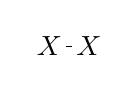
\begin{tikzpicture}[baseline={([yshift=-.5ex]current bounding box.center)}]
    \path (0,0) node (A) {$X$} ++ (0.5,0) node (B) {$X$};
    \draw (A) -- (B);
\end{tikzpicture}
\end{align}

We choose a particular 1-element set $\{*\}$ that acts as the identity in the sense that $\{*\}\times A\cong A\times \{*\} \cong A$ for any set $A$. The erase map $\text{del}_X:X\kto \{*\}$ defined by $(\text{del}_X)(*|x) = 1$ is a Markov kernel that ``discards the input''. It is drawn as a fuse:

\begin{align}
    \text{del}_X&:=\begin{tikzpicture}[baseline={([yshift=-.5ex]current bounding box.center)}]
    \path (0,0) ++ (1,0) node (B) {$X$};
    \draw[-{Rays[n=8]}] (A) -- (B);
\end{tikzpicture}
\end{align}

The copy map $\text{copy}_X:X\kto X\times X$ defined by $(\text{copy}_X)(x',x''|x)=\llbracket x=x' \rrbracket \llbracket x=x'' \rrbracket$ is a Markov kernel that makes two identical copies of the input. It is drawn as a fork:

\begin{align}
    \text{copy}_X&:=\begin{tikzpicture}[baseline={([yshift=-.5ex]current bounding box.center)}]
    \path (0,0) node (A) {$X$} 
    ++ (0.5,0) node[copymap] (copy0) {}
    ++ (0.5,0.15) node (B) {$X$}
    + (0,-0.3) node (C) {$X$};
    \draw (A) -- (copy0) to [out=45,in=180] (B) (copy0) to [out=-45, in=180] (C);
\end{tikzpicture}
\end{align}

The swap map $\text{swap}_{X,Y}:X\times Y\kto Y\times X$ defined by $(\text{swap}_{X,Y})(y',x'|x,y)=\llbracket x=x' \rrbracket\llbracket y=y' \rrbracket$ swaps two inputs, and is represented by crossing wires:

\begin{align}
    \text{swap}_X &:=  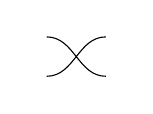
\begin{tikzpicture}[baseline={([yshift=-.5ex]current bounding box.center)}]
        \path (0,0) node (A) {} 
        + (0,-0.5) node (B) {}
        ++ (1,0) node (C) {}
        + (0,-0.5) node (D) {};
        \draw (A) to [out=0,in=180] (D) (B) to [out=0, in=180] (C);
    \end{tikzpicture}
\end{align}

Because we anticipate that the graphical notation will be unfamiliar, we will include some examples in the next section.

\subsubsection{Examples}

When translating string diagram notation to integral notation, a number of identities can speed up the process.

For arbitrary $\kernel{K}:X\times Y\to Z$, $\kernel{L}:W\to Y$

\begin{align}
 [(\text{id}_X\otimes \kernel{L})\kernel{K}](A|x,w) &= \int_{Y}\int_X   \kernel{K}(z|x',y')\kernel{L}(dy'|w)\text{id}_X(dx'|x)\\
                                           &= \int_Y  \kernel{K}(z|x,y') \kernel{L}(dy'|w)
\end{align}

That is, an identity map passes its input to the next kernel in the product. 

For arbitrary $\kernel{K}: X\times Y\times Y\to Z$ (where we apply the above shorthand in the first line):

\begin{align}
 [(\text{id}_X\otimes \text{copy}_Y)\kernel{K}](A|x,y) &= \int_Y\int_Y \kernel{K}(A|x,y',y'') \text{copy}_Y(dy'\times dy''|y)\\
                                           &= \kernel{K}(A|x,y,y)
\end{align}

That is, the copy map passes along two copies of its input to the next kernel in the product. 

For a collection of kernels $\kernel{K}^n:Y^n\to Z$, $n\in[n]$, define $(y)^{n}=(y|i\in[n])$ and:

\begin{align}
    \text{copy}^n_Y &:= \begin{cases}
    \text{copy}^{n-1}_Y(\text{id}_{Y^{n-2}}\otimes \text{copy}_Y) & n>2\\
    \text{copy}_Y & n=2
    \end{cases}\\
    (\text{copy}^2_Y\kernel{K}^2)(z|y) &= \kernel{K}^2(z|y,y)\\
\end{align}

Suppose for induction
\begin{align}
(\text{copy}^{n-1}_Y\kernel{K}^{n-1})(z|y) &= \kernel{K}^{n-1}(z|(y)^{n-1})
\end{align}

then
\begin{align}
(\text{copy}^n_Y\kernel{K}^n)(z|y) &= (\text{copy}^{n-1}_Y(\text{id}_{Y^{n-2}}\otimes \text{copy}_Y)\kernel{K}^n)(z|y)\\
                                     &= \sum_{y'\in Y^{n-1}}(\text{id}_{Y^{n-2}}\otimes \text{copy}_Y)(\mathbf{y}'|(y)^{n-1})\kernel{K}^n(z|\mathbf{y}')\\
                                     &= \kernel{K}^n(z|(y)^n)
\end{align}

That is, we can define the $n$-fold copy map that passes along $n$ copies of its input to the next kernel in the product.

\subsubsection{Example: comb insertion}

The following examples illustrate 2-combs and the insertion operation, both of which we will define later. As an example in translating diagrams, we show how the diagrams for a 2-comb and 2-comb with an inserted Markov kernel can be translated to integral notation.

Consider the Markov kernels $\kernel{K}:W\kto X$, $\kernel{L}:X\times W\times Y\kto Z$ and the 2-comb $\kernel{M}:W\times Y\kto X\times Z$ defined as

\begin{align}
    \kernel{M} = \tikzfig{2_comb}\label{eq:2comb_M}
\end{align}

Following the rules above, we can translate this to ordinary notation by first breaking it down into products and tensor products, and then evaluating these products

\begin{align}
    \kernel{M}(A\times B|w,y) = [&(\text{copy}_W\otimes \text{id}_Y)(\kernel{K}\otimes \text{id}_{W\times Y})\\
    &(\text{copy}_X\otimes \text{id}_{W\times Y})(\text{id}_X\otimes\kernel{L})](A\times B|w,y)\\
                        = [&(\kernel{K}\otimes \text{id}_{W\times Y})(\text{copy}_X\otimes \text{id}_{W\times Y})\\
                        &(\text{id}_X\otimes\kernel{L})](A\times B|w,w,y)\\
                        = \;&\int_{X}  (\text{id}_X\otimes\kernel{L})(A\times B|x',w,y) \kernel{K} (dx'|w)
                        ](y,z|y',x)\\
                        = \;&\int_X \text{id}_X(A|x') \kernel{L}(B|x',w,y)\kernel{K}(dx'|w)\\
                        = \;&\int_A \kernel{L}(B|x',w,y)\kernel{K}(dx'|w)
\end{align}

If we are given additionally $\kernel{J}:X\times W\kto Y$, we can define a new Markov kernel $\kernel{N}:W\kto Z$ given by ``inserting'' $\kernel{J}$ into $\kernel{M}$:

\begin{align}
    \kernel{N} = \tikzfig{2comb_inserted_anon}\label{eq:2comb_winsert}
\end{align}


We can translate Equation \ref{eq:2comb_winsert} to

\begin{align}
    \kernel{N}(A\times B\times C|w) = &[\text{copy}_W(\kernel{K}\text{copy}^3_Y\otimes \text{id}_W)\\
    &(\text{id}_Y\otimes\kernel{J}\otimes \text{id}_Y)(\text{id}_Y \otimes \text{copy}_X\otimes \text{id}_Y)\\
    &(\kernel{L}\otimes \text{id}_X\otimes \text{id}_Y)] (A\times B\times C|w)\\
                    = &[(\kernel{K}\text{copy}^3_Y\otimes \text{id}_W)(\text{id}_Y\otimes\kernel{J}\otimes \text{id}_Y)\\
                    &(\text{id}_Y \otimes \text{copy}_X\otimes \text{id}_Y)\\
                    &(\kernel{L}\otimes \text{id}_X\otimes \text{id}_Y)] (A\times B\times C|w,w)\\
                    = &\int_X\int_Y\kernel{L}(C|x',w,y') \text{id}_X(A|x') \text{id}_Y(B|y') \kernel{J}(dy'|x',w)\kernel{K}(dx'|w)\\
                    = &\int_A\int_B\kernel{L}(C|x',w,y') \kernel{J}(dy'|x',w)\kernel{K}(dx'|w)
\end{align}
